\Transcb{yellow}{blue}{Gravity as a geometrical effect}
\onecolumn
\begin{itemize}
\item Deflection of light in a gravitational field
\item[] Not corresponding to Newtonian gravity formula
\item[] Ultimate proof that all particles experience the same $\vec{a}$ irrespective of $m$
\item Einstein's idea concerning gravitational path deflection
\item[] Consider a particle traveling in a straight line over a flat rubber sheet
\item[] Put a heavy object on the rubber sheet $\rightarrow$ sheet stretches and curves
\item[] $\rightarrow$ The particle will now follow a curved path on the sheet
\item[] {\blue Gravitational path deflection is due to curvature of space}
\item Similar reasoning for the time coordinates
\item[] {\blue Gravitational time dilation is due to curvature of time}
\end{itemize}
%
\begin{center}
\colorbox{yellow}{Relativistic viewpoint on gravity}\\[3mm]
{\red \shabox{Gravity is a geometric effect due to curvature of space-time}}\\[3mm]
{\red \shabox{The presence of mass introduces a curvature in space-time}}
\end{center}

\Tr
\begin{center}
{\blue Curvature of space due to the presence of mass}\\[5mm]
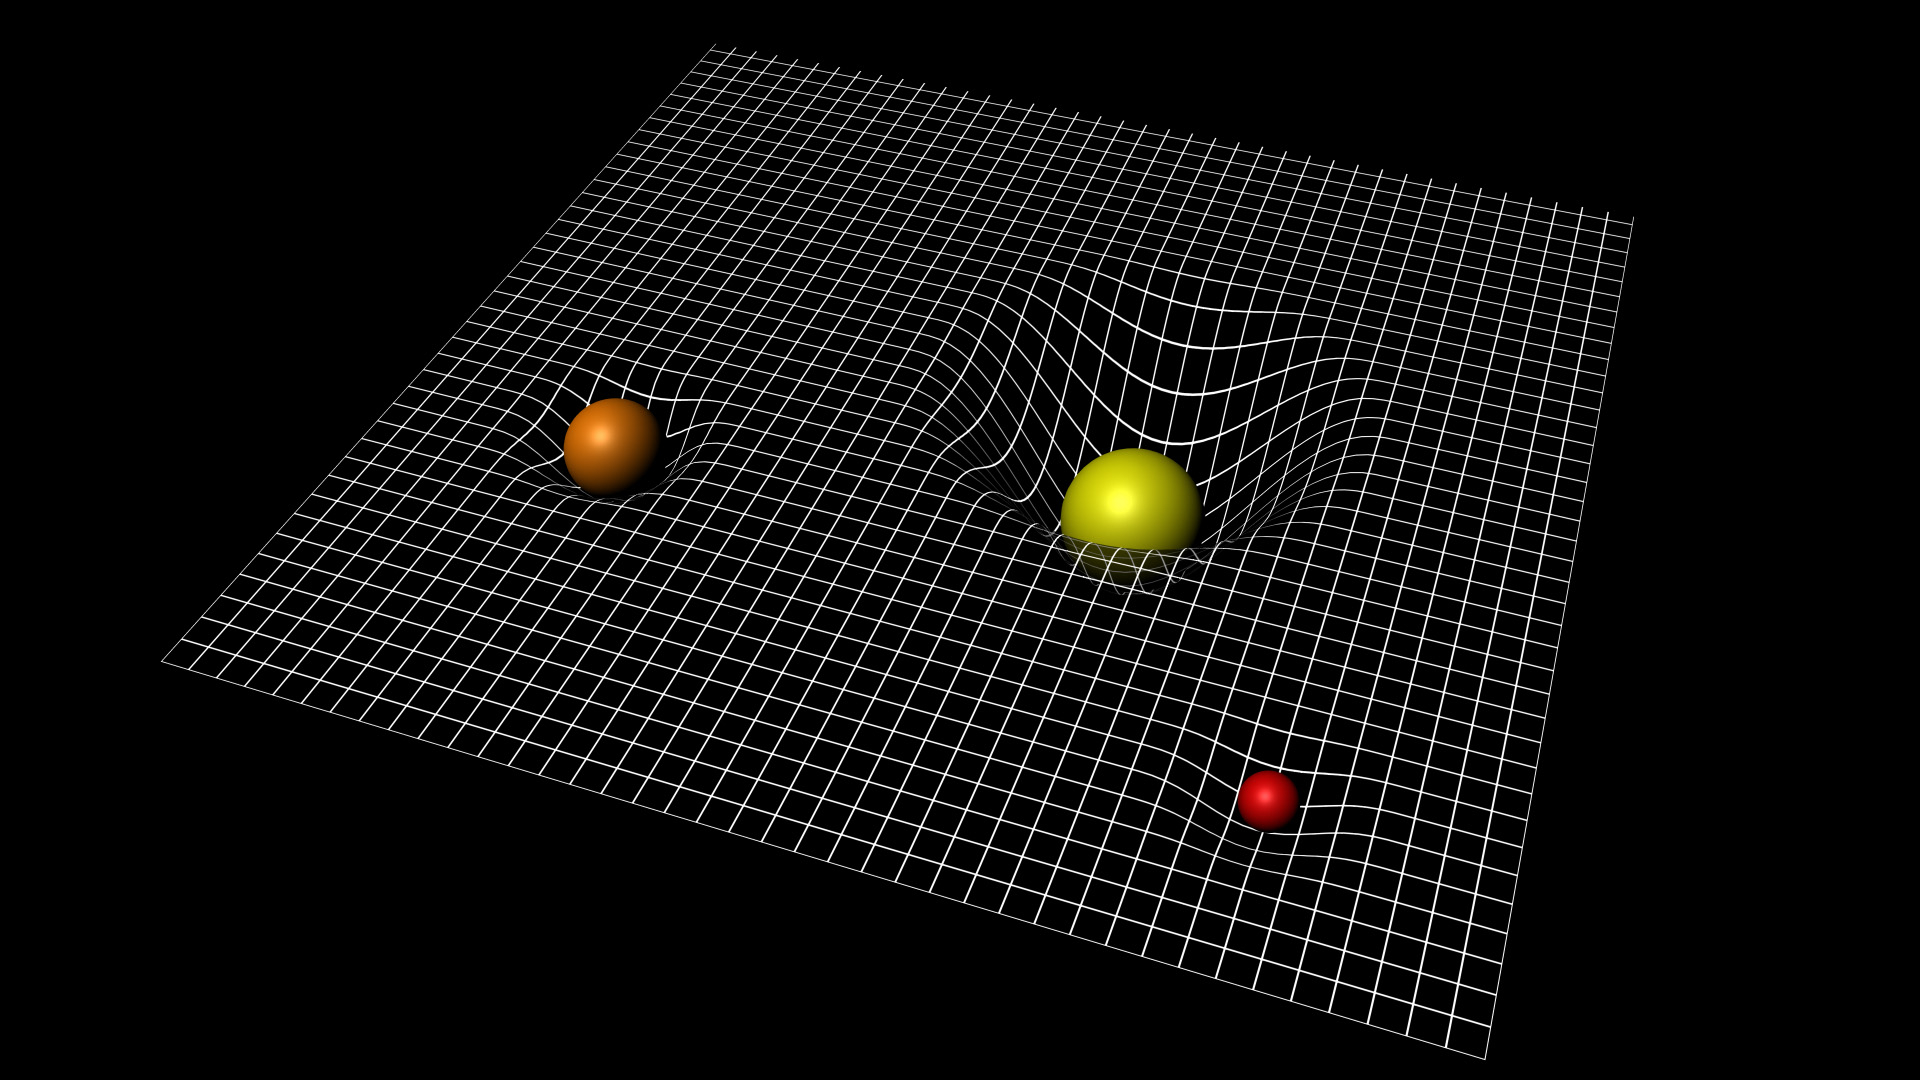
\includegraphics[keepaspectratio,height=14cm]{curvature}
\end{center}

\Tr
\twocolumn[\begin{center}{\blue Gravitational lensing}\end{center}]
%
\begin{center}
The principle\\[3mm]
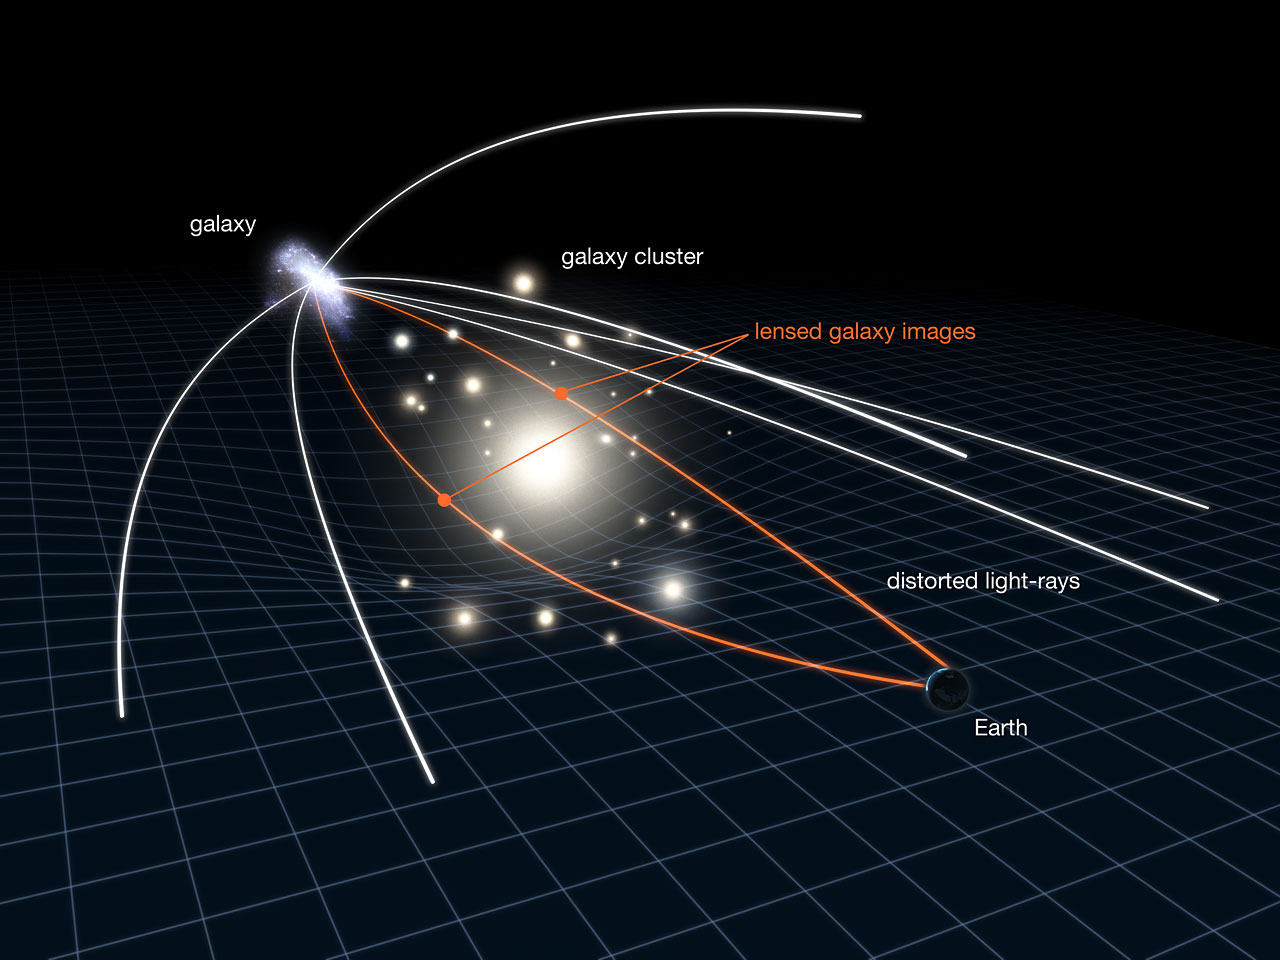
\includegraphics[keepaspectratio,width=14cm]{grav-lens}
\end{center}

\newpage
%
\begin{center}
An observation\\[3mm]
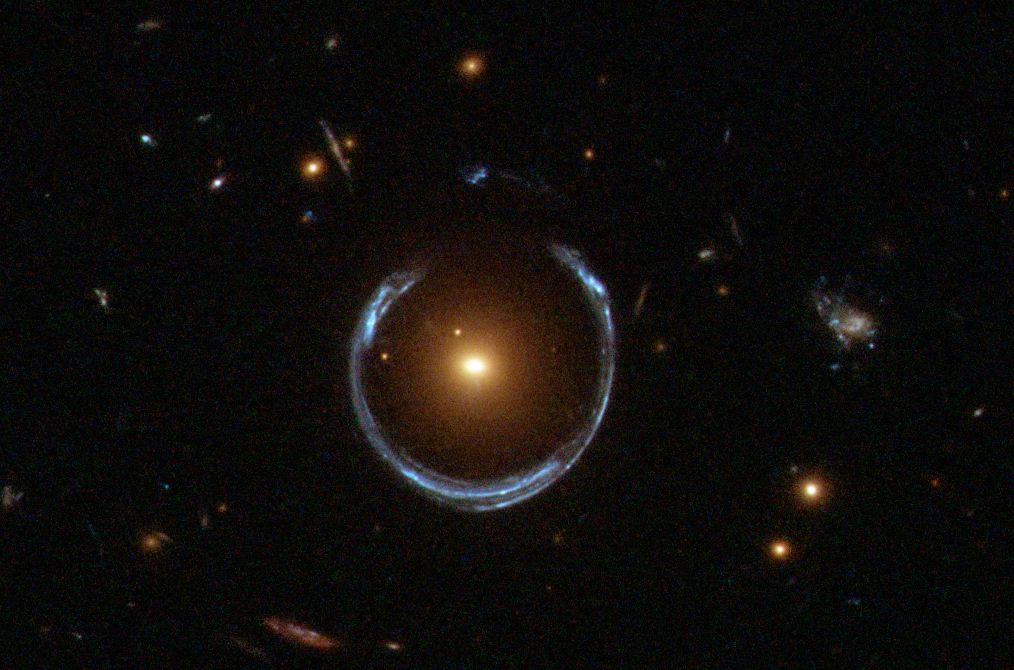
\includegraphics[keepaspectratio,width=12cm]{grav-ring}
\end{center}

\Tr
\onecolumn
\begin{center}
{\blue Gravitational Waves}
\end{center}
%
\begin{itemize}
\item Consider 2 heavy objects rotating closely around each other
\item[] Time dependent space-time deformations cause ripples (e.g. a water surface)
\item[] $\rightarrow$ These are called {\red gravitational waves}
\item Frequency of the gravitational wave is related to the orbital period
\item[] Shorter orbital period $\rightarrow$ Higher frequency (shorter wavelength)
\end{itemize}
%
\begin{center}
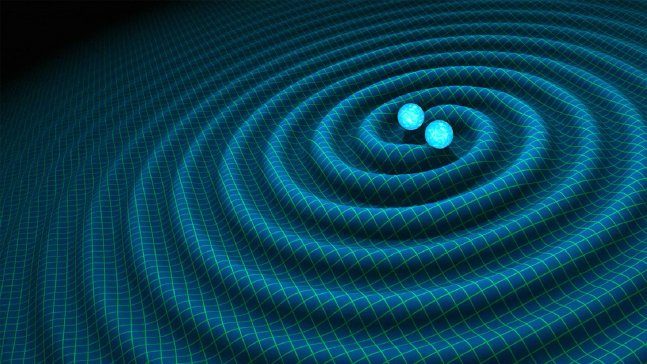
\includegraphics[keepaspectratio,height=8cm]{spiral-waves}
\end{center}

\Tr
\twocolumn[\begin{center}{\blue A first indication : The binary pulsar PSR B1913+16}\end{center}]
%
\begin{center}
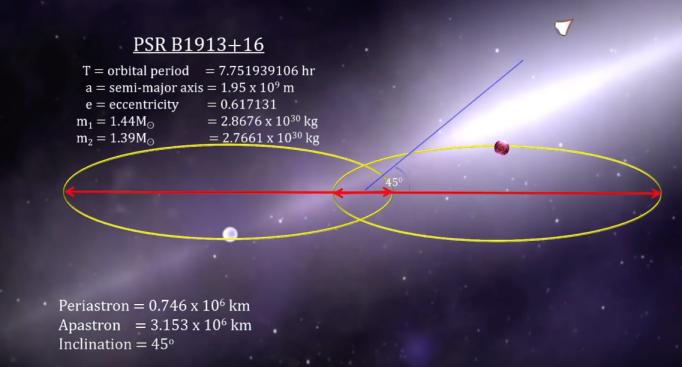
\includegraphics[keepaspectratio,width=15cm]{Hulse-Taylor-psr}
\end{center}
%
\begin{itemize}
\item In case of emission of gravitational waves
\item[] $\rightarrow$ Loss of energy
\item[] $\rightarrow$ Change of orbital period
\item Observe a decrease of the orbital period ?
\end{itemize}


\newpage

\begin{center}
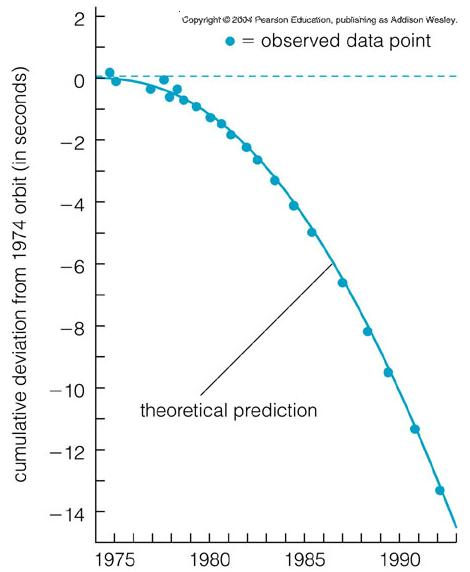
\includegraphics[keepaspectratio,width=10cm]{Hulse-Taylor-curve}\\[3mm]
{\blue Russel Hulse and Joe Taylor\\
Nobel prize  1993}
\end{center}
\Tr
\twocolumn[\begin{center}{\red The discovery of gravitational waves (2015)}\end{center}]
%
\begin{itemize}
\item Gravitational wave deforms space
\item[] $\rightarrow$ Temporary change $\Delta L$
\item Example : 2 corks at a water surface
\end{itemize}
%
\begin{center}
{\blue The detection principle}\\[3mm]
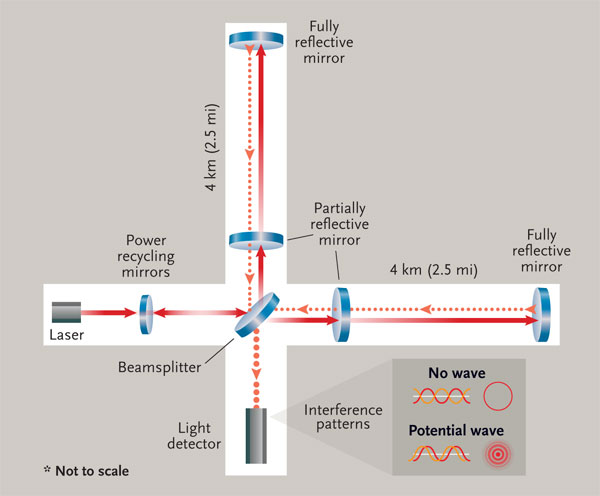
\includegraphics[keepaspectratio,width=11cm]{LIGO-schematic}
\end{center}

\newpage
%
\begin{center}
{\blue The Ligo and Virgo interferometers}\\[3mm]
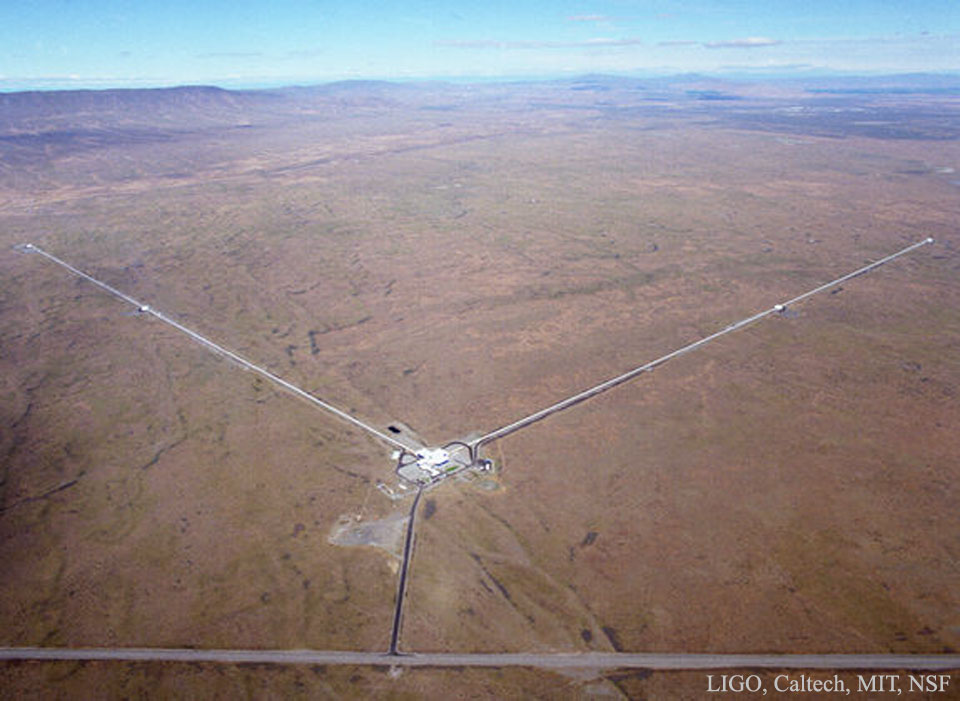
\includegraphics[keepaspectratio,width=12cm]{hanford-ligo}
\end{center}
%
\begin{itemize}
\item[] Ligo: Hanford (WA), Livingston (LA)
\item[] Virgo: Cascina (Italie)
\end{itemize}

\Tr
\twocolumn[\begin{center}{\red A subtle interplay}\end{center}]
%
\begin{itemize}
\item[] \begin{center}{\blue Noise reduction and arrival direction}\end{center}
\item Hanford-Livingston: $\sim$3000 km
\item Grav. wave moves with light speed
\item Timing of the  coincidence
\item[] $\rightarrow$ Reduces noise
\item[] $\rightarrow$ Provides arrival direction
\end{itemize}
%
\begin{center}
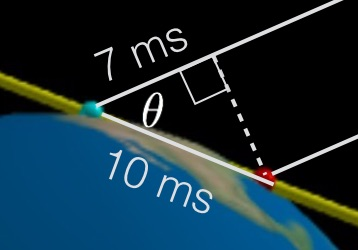
\includegraphics[keepaspectratio,width=10cm]{ligo-dt}
\end{center}

\newpage
%
\begin{center}
{\blue The discovery (GW150914)}\\[3mm]
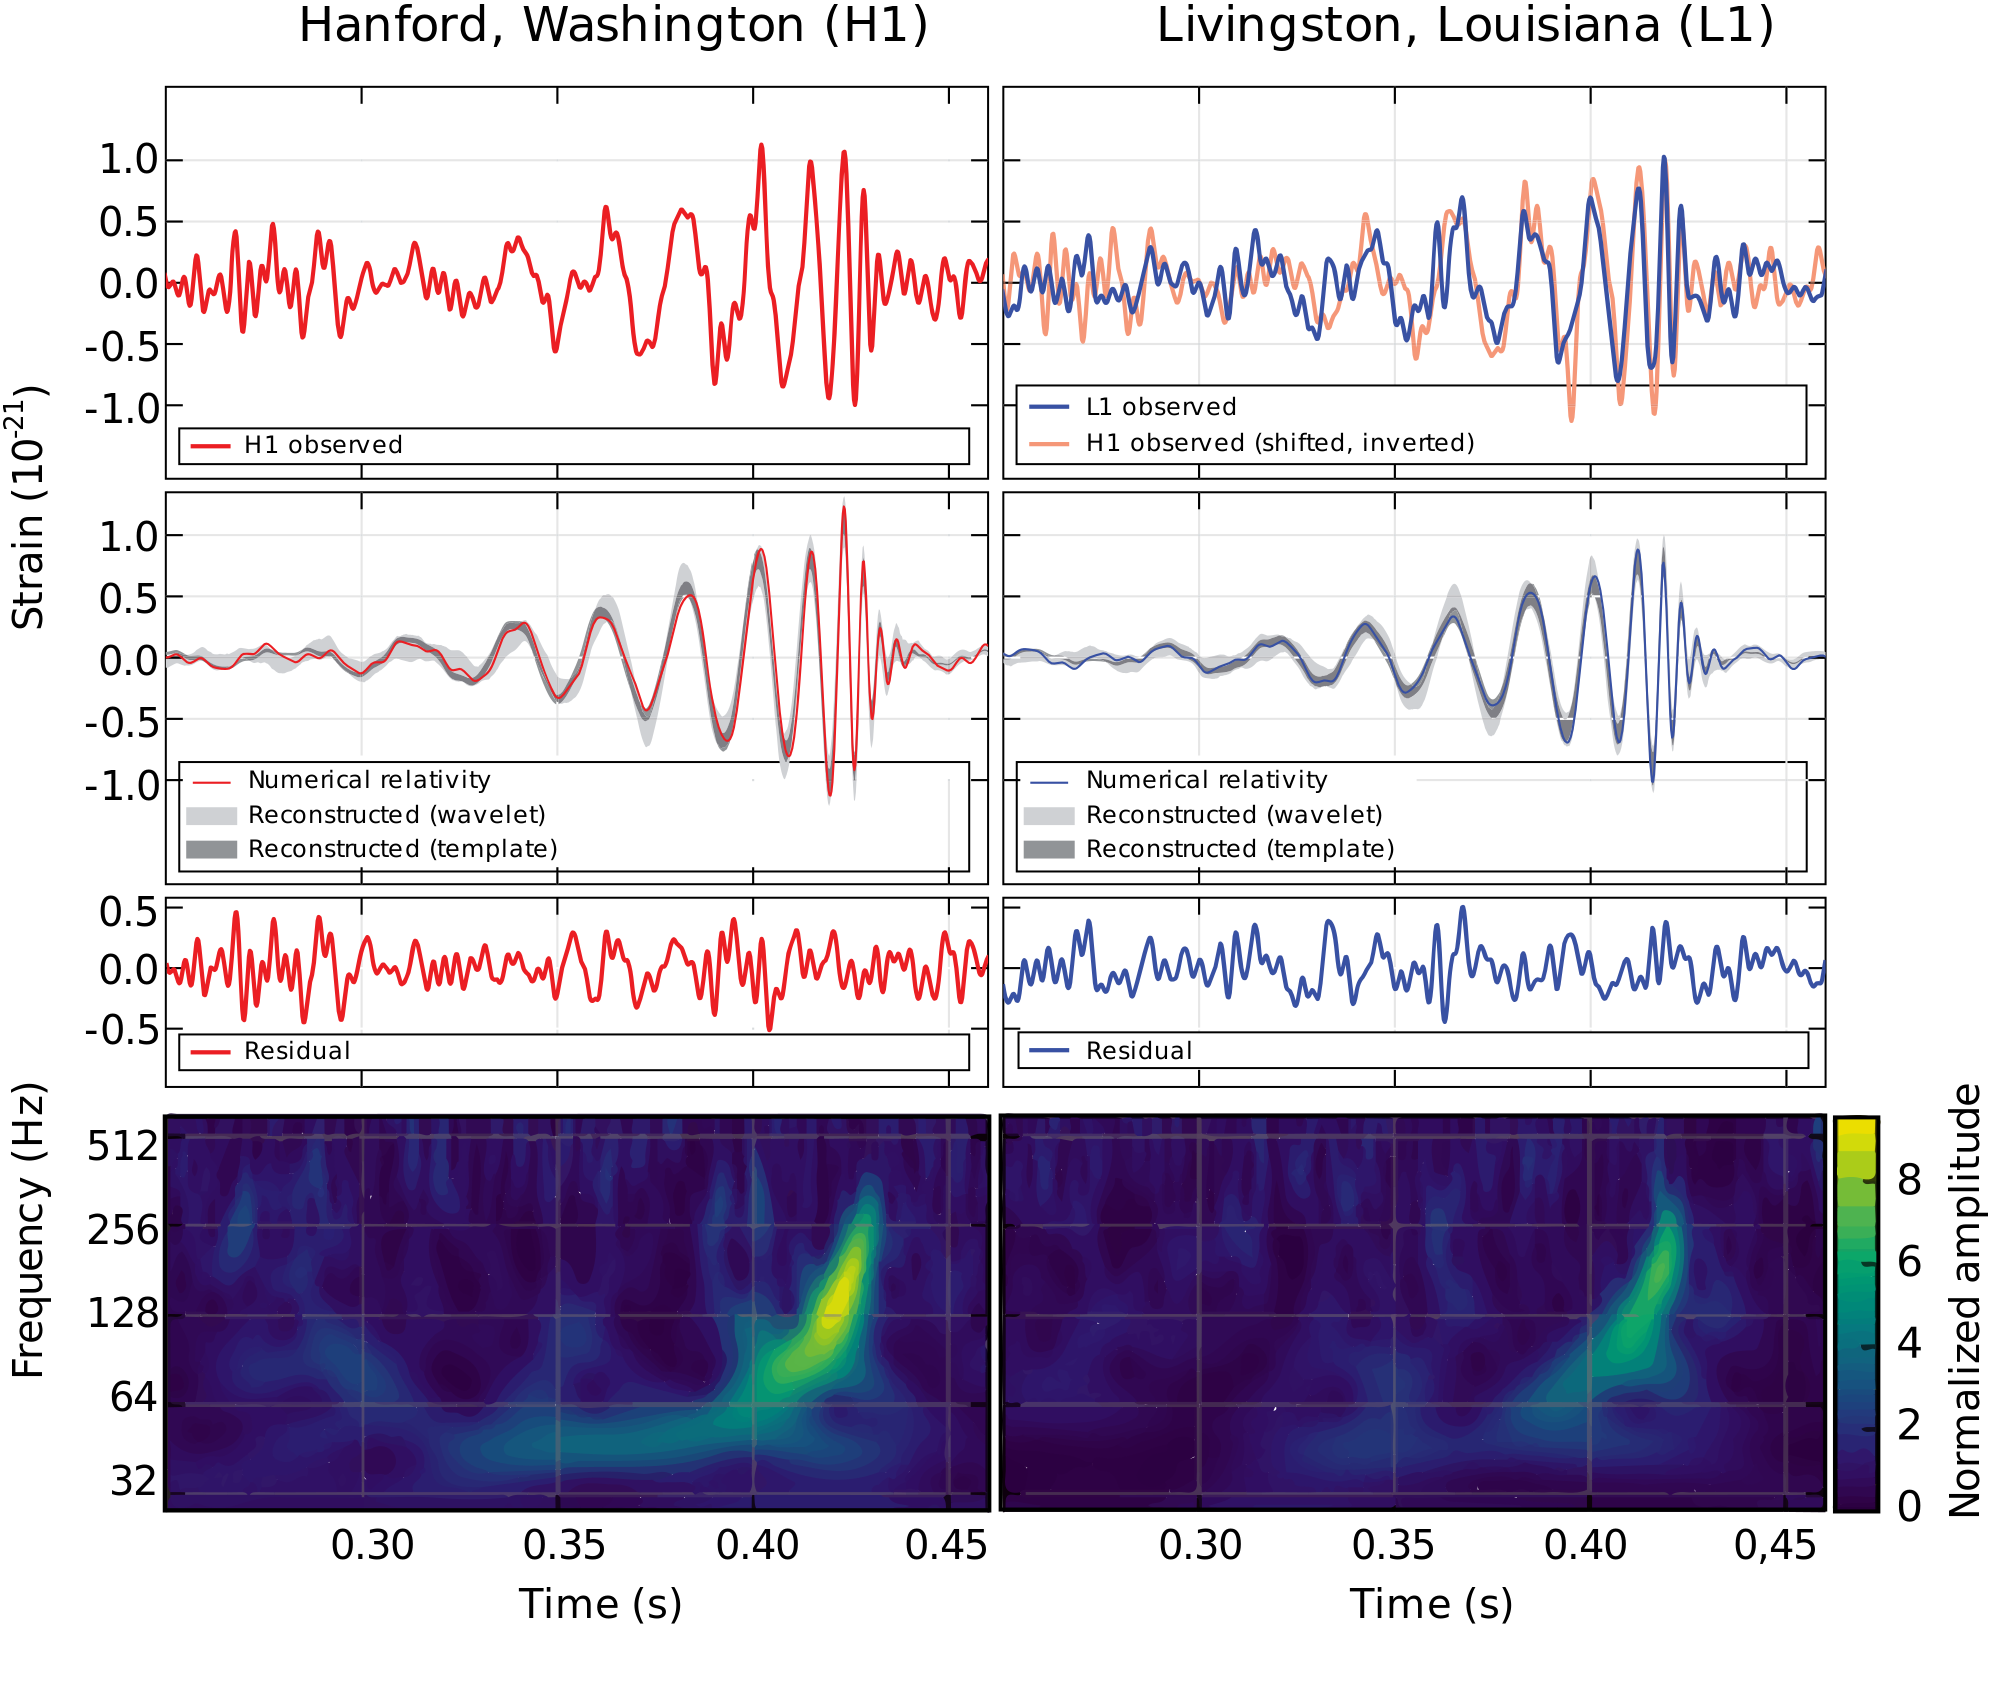
\includegraphics[keepaspectratio,width=15cm]{GW150914}
\end{center}

\Tr
\onecolumn
\begin{itemize}
\item[] \begin{center}{\blue Analysis of GW150914}\end{center}
\item Try to describe the observed pattern on basis of theoretical templates
\item[] $\rightarrow$ 2 Black Holes with $M_{1} \approx 30M_{\odot} \quad M_{2} \approx 35M_{\odot}$ and $M_{end} \approx 62M_{\odot}$
\item[] $\rightarrow$ An energy equivalent of $3M_{\odot}c^{2}$ has been emitted in a fraction of a second !
\item[] $P_{max} \approx 3.6 \cdot 10^{49}$W $\rightarrow$ More than all stars in the visible Universe !
\item Distance ca. 440 Mpc ($\sim 1.3 \cdot 10^{9}$ light year)
\end{itemize}
%
\begin{center}
{\red \shabox{Nobel prize 2017 for the discovery of gravitational waves}}\\
(Barry Barish, Kip Thorne en Rainer Weiss)
\end{center}

\Tr
\twocolumn[\begin{center}
            {\blue How to introduce curvature in space-time in accordance with observations ?}
            \vspace*{3mm}
           \end{center}]
\begin{itemize}
\item Detailed look at the equivalence principle
\item[] Frame $S$ in free fall with two objects at rest
\item[$\ast$] {\red Can the earth gravity stay "hidden" ?}
\item[] $|\vec{g}|$ must be constant in $S \rightarrow \d y$ small
\item[] $g_{x}$ must be small $\rightarrow \d x$ small
\item[] Observation time $T$ must be small
\item[] \begin{center}\colorbox{yellow}{The Equivalence Principle}\end{center}
{\red
\item[] Experiments performed in a sufficiently\\
        small freely falling laboratory, over a\\
        sufficiently short time, yield results that are\\
        indistinguishable from those of the same\\
        experiments performed in an inertial frame in empty space.
}
\end{itemize}

\newpage

\begin{center}
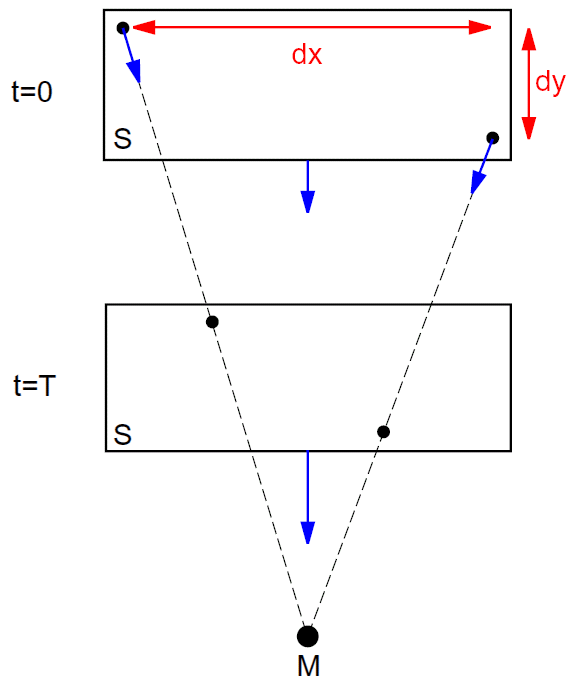
\includegraphics[keepaspectratio,height=14cm]{equivalence2}
\end{center}

\Tr
\twocolumn[\begin{center}
            {\blue Linking the Equivalence Principle with relativity}
            \vspace*{5mm}
           \end{center}]
%
\begin{itemize}
\item Relativistic description of an {\red inertial frame}
\item[] It's all included in the metric
\item[] $\d s^{2}=(c\d t)^{2}-\d\vec{r}^{\,2}$
\item[] As 4-vectors~: {\red $\d s^{2}=\eta_{\mu\nu}\,\d x^{\mu}\,\d x^{\nu}$}
\item[] with $\eta_{\mu\nu}=\text{diag}(1,-1,-1,-1)$
\item In the presence of gravity~:
\item[] Freely falling frame is only locally inertial
\item[] $\rightarrow$ All other locations in space-time have~:
\item[] {\blue $\qquad \d s^{2}=g_{\mu\nu}(\Fvec{x})\,\d x^{\mu}\,\d x^{\nu}$}
\item[] $\Fvec{x} \equiv$ location in space-time
\end{itemize}

\newpage

\begin{itemize}
\item[] \begin{center}\colorbox{yellow}{Description of space-time curvature}\end{center}
{\red
\item[] Introduce metric tensor $g_{\mu\nu}(\Fvec{x})$ of which the components
        depend on the location in space-time 
}
\item Equivalence Principle~: $S \rightarrow S^{\,\prime}$
\item[] $g_{\mu\nu}(\Fvec{x}) \rightarrow g_{\mu\nu}^{\,\prime}(\Fvec{x}^{\,\prime})=\eta_{\mu\nu}$
\item Consequences~:
{\blue
\item[] $g_{\mu\nu}(\Fvec{x})$ must be a symmetric 4x4 matrix
\item[] Always 1 time and 3 space coordinates
}
\item[$\ast$] This is the basis of {\red General Relativity}
\item[] \colorbox{yellow}{What are the components of $g_{\mu\nu}(\Fvec{x})$ ?}
\item[] $\rightarrow$ Need to investigate curvature
\end{itemize}